\documentclass[10pt]{beamer}

\usetheme[progressbar=frametitle]{metropolis}
\usepackage{appendixnumberbeamer}

\usepackage{booktabs}
\usepackage{svg}
\usepackage[scale=2]{ccicons}

\usepackage{pgfplots}
\usepgfplotslibrary{dateplot}

\usepackage{xspace}
\newcommand{\themename}{\textbf{\textsc{metropolis}}\xspace}
\usetikzlibrary{positioning}

\title{Finite Statemachines}
\subtitle{Specify and Implement dynamic Behaviour}
\date{\today}
\author{Stefan Dennig}
\institute{NewTec GmbH}
% \titlegraphic{\hfill\includegraphics[height=1.5cm]{logo.pdf}}

\begin{document}
\metroset{block=fill}
\maketitle

\section[Example]{Example}

\begin{frame}[fragile]{Example Button Debounce}
  \begin{columns}[T,onlytextwidth]
    \column{0.5\textwidth}
    Button Debounce Statemachine
    \begin{itemize}
      \item Button Inactive - Button is registered as released
      \item Button pressed - latch event after first pressed
      \item Button active - Button is registered as pressed
      \item Button released - latch event after first release
    \end{itemize}
    \column{0.5\textwidth}
      \begin{center}
        \includegraphics[keepaspectratio,scale=0.35]{out/Statemachine.png}
      \end{center}
  \end{columns}
\end{frame}

\section[Theory]{Finite Statemachine}

\begin{frame}[fragile]{Definition}
  \begin{block}{Definition of a Statemachine}
    A finite-state machine (FSM) is a mathematical model of computation. 
    It is an abstract machine that can be in exactly one of a finite number of states at any given time. 
    The FSM can change from one state to another in response to some inputs; 
    the change from one state to another is called a transition.
  \end{block}
\end{frame}

\begin{frame}[fragile]{Definition}
  \begin{columns}[T,onlytextwidth]
    \column{0.5\textwidth}
      Parameters of a Statemachine:
      \begin{itemize}
        \item states $s$
        \item transitions $t$
        \item event $\sigma$
      \end{itemize}
      \begin{center}
      \begin{equation*}
        s \in \bold{S}
      \end{equation*}
    \end{center}
    \column{0.5\textwidth}
        \begin{block}{Definition of State}
          The state of a system is defined by the smallest possible number of its changeable internal parameters.
          e.g.: 
          \begin{itemize}
            \item velocity
            \item position
            \item temperature
          \end{itemize}
        \end{block}
    \end{columns}
\end{frame}

\begin{frame}[fragile]{Definition}
  \begin{columns}[T,onlytextwidth]
    \column{0.5\textwidth}
      Parameters of a Statemachine:
      \begin{itemize}
        \item states $s$
        \item transitions $t$
        \item event $\sigma$
      \end{itemize}
      \begin{center}
      \begin{equation*}
        t \in \bold{T}
      \end{equation*}
      \end{center}

    \column{0.5\textwidth}
        \begin{block}{Definition of Transition}
          A Transition is a change from one set of paramaters of a system to another one. 
          e.g.: 
          \begin{itemize}
            \item acceleration
            \item heat
          \end{itemize}
        \end{block}
    \end{columns}
\end{frame}

\begin{frame}[fragile]{Definition}
  \begin{columns}[T,onlytextwidth]
    \column{0.5\textwidth}
      Parameters of a Statemachine:
      \begin{itemize}
        \item states $s$
        \item transitions $t$
        \item event $\sigma$
      \end{itemize}
      \begin{center}
      \begin{equation*}
        \sigma \in \bold{\Sigma}
      \end{equation*}
      \end{center}

    \column{0.5\textwidth}
        \begin{block}{Definition of Event}
          A Event is a change of inputs of a system.
          e.g.: 
          \begin{itemize}
            \item push of gas pedal
            \item expiration of time
          \end{itemize}
        \end{block}
    \end{columns}
\end{frame}

\begin{frame}[fragile]{Definition}
  \begin{block}{Finite}
    A finite Statemachine only implements a limited set of states $\bold{S}$. This implicates a limited set of transitions $\bold{T}$ and a limited set of Events $\bold{E}$
  \end{block}

  A Statemachine can be described as a set functions $t$ operating on its internal state $s$. The output $y$ depends on the internal state $s$, additionaly it may depend on the input $\sigma$.
  \begin{center}
  \begin{equation}
    s_{n+1} = t(s_n,\sigma)
  \end{equation}
  \begin{equation}
    \lambda = g(s_n,\sigma)
  \end{equation}
  \end{center}
\end{frame}

\begin{frame}[fragile]{Facts}
 \begin{itemize}
  \item Statemachines, as per Definition, do not imply any timing behaviour.
  \item Every Memory implicitly holds state, thus implements a statemachine.
  \item The amount of states is proportional to the complexity of the statemachine.
  \item Every slightly complex component implements a statemachine.
 \end{itemize}
\end{frame}

\begin{frame}[fragile]{Design of Statemachines}
When to use a statemachine?
 \begin{itemize}
  \item Simple Behaviour that can be clustered
  \item Strict Deterministic control
  \item Ressource/Device Control
 \end{itemize}
When not to use a statemachine?
 \begin{itemize}
  \item If a combinational logic is an alternative
  \item If a mathematical formula can be used instead (filters)
  \item Multiple Statemachines should never implement the same state
 \end{itemize}
  \begin{alertblock}{Senior Experience}
    State should be avoided.
  \end{alertblock}
\end{frame}

\begin{frame}[fragile]{Designtips}
 \begin{itemize} 
  \item Decide about timing (cyclic, synchronous, asynchronous)
  \item Number of states shall be reduced
  \item Hierarchical Statemachines are a good way to reduce states
  \item Statemachines that are directly or indirectly linked shall be avoided
  \item Make states explicit (no rotation direction as variable, no global variables)
  \item If a component implies state implement it as a statemachine (init, running, error)
  \item shall invalid transitions be neglected or treated as errors?
 \end{itemize}

  \begin{alertblock}{Senior Experience}
    Do not hide difficulties. Put them in a place to handle them.
  \end{alertblock}
\end{frame}

\begin{frame}[fragile]{Questions}
\begin{itemize}
\item How many states does a Integer(8-Bit) hold?
\item How many states can a microcontroller with $2$ KBytes of RAM and $16$KBytes of ROM have?
\item What is the maximum amount of transitions in a state machine with $4$ States?
\end{itemize}
\end{frame}

\begin{frame}[fragile]{Questions}
\begin{itemize}
\item How many states does a Integer(8-Bit) hold? $\bold{256}$
\item How many states can a microcontroller with 2KBytes of RAM and 16KBytes of ROM have? $\bold{2^{18000}}$
\item What is the maximum amount of transitions in a state machine with $4$ States? $\bold{16}$
\end{itemize}
\end{frame}

\section[Implementation]{Implementation}

\begin{frame}[fragile]{Mealy Machine}
  \begin{center}
      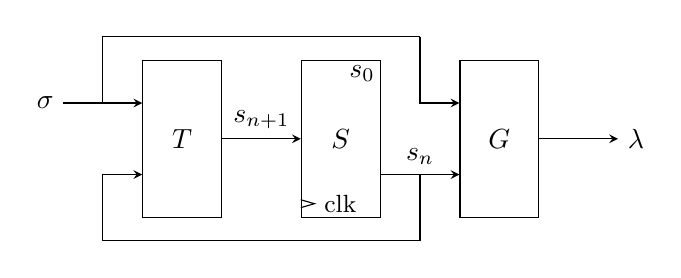
\begin{tikzpicture}
      \node [draw, minimum width=1cm, minimum height=2cm]  (input_logic) {$\bold{T}$};
      \node [draw, minimum width=1cm, minimum height=2cm, right=1cm of input_logic]  (memory) {$\bold{S}$};
      \node [draw, minimum width=1cm, minimum height=2cm, right=1cm of memory]  (output_logic) {$\bold{G}$};
      \node [below=0.33cm of input_logic.west]  (input_logic_state_in) {};
      \node [above=0.33cm of input_logic.west]  (input_logic_in_in) {};
      \node [above=0.33cm of output_logic.west]  (output_logic_in_in) {};
      \node [below=0.33cm of output_logic.west]  (output_logic_state_in) {};
      \node [below=0.33cm of memory.east]  (state_out) {};

      \draw [-stealth] (input_logic.east) -- (memory.west) node[midway,above]{$s_{n+1}$};
      \draw [-stealth] (state_out.center) -- (output_logic_state_in.center) node[midway] (state) {} node[midway,above] {$s_{n}$};
      \draw [stealth-] (input_logic_in_in.center) -- ++(-1,0) node[midway] (helper1) {} node[behind path, left]{$\sigma$};
      \draw [-stealth] (output_logic.east) -- ++(1,0) node[behind path, right]{$\lambda$};

      \node [below=1.5cm of helper1]  (helper2) {};
      \node [above=1.5cm of state]  (helper3) {};
      
      \draw (state.center) |- (helper2.center);
      \draw [-stealth] (helper2.center) |- (input_logic_state_in.center);
      \draw (helper1.center) |- (helper3.center);
      \draw [-stealth] (helper3.center) |- (output_logic_in_in.center);

  \node [below=0.75cm of memory.west]  (tri_a) {};
  \node [below=0.70cm of memory.west]  (tri_b_) {};
  \node [right=0.05cm of tri_b_.center]  (tri_b) {};
  \node [right=0.00cm of tri_b.center] (clock) {{\small clk}};
  \node [below=0.65cm of memory.west]  (tri_c) {};
  \draw (tri_a.center) -- (tri_b.center)  -- (tri_c.center);

  \node [below=0.05cm of memory.north east]  (s0_) {};
  \node [left=-0.05cm of s0_.center]  (s0) {$s_0$};

    \end{tikzpicture}

  \end{center}
  \begin{center}
  \begin{equation}
    s_{n+1} = t(s_n,\sigma)
  \end{equation}
  \begin{equation}
    \lambda = g(s_n,\sigma)
  \end{equation}
  \end{center}
\end{frame}

\begin{frame}[fragile]{Moore Machine}

\begin{center}
  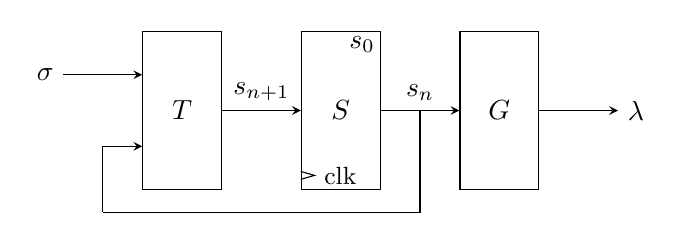
\begin{tikzpicture}

  \node [draw, minimum width=1cm, minimum height=2cm]  (input_logic) {$\bold{T}$};
  \node [draw, minimum width=1cm, minimum height=2cm, right=1cm of input_logic]  (memory) {$\bold{S}$};
  \node [draw, minimum width=1cm, minimum height=2cm, right=1cm of memory]  (output_logic) {$\bold{G}$};
  \node [below=0.33cm of input_logic.west]  (input_logic_state_in) {};
  \node [above=0.33cm of input_logic.west]  (input_logic_in_in) {};

  \draw [-stealth] (input_logic.east) -- (memory.west) node[midway,above]{$s_{n+1}$};
  \draw [-stealth] (memory.east) -- (output_logic.west) node[midway] (state) {} node[midway,above] {$s_{n}$};
  \draw [stealth-] (input_logic_in_in.center) -- ++(-1,0) node[midway] (helper1) {} node[behind path, left]{$\sigma$};
  \draw [-stealth] (output_logic.east) -- ++(1,0) node[behind path, right]{$\lambda$};

  \node [below=1.5cm of helper1]  (helper2) {};
  
  \draw (state.center) |- (helper2.center);
  \draw [-stealth] (helper2.center) |- (input_logic_state_in.center);

  \node [below=0.75cm of memory.west]  (tri_a) {};
  \node [below=0.70cm of memory.west]  (tri_b_) {};
  \node [right=0.05cm of tri_b_.center]  (tri_b) {};
  \node [right=0.00cm of tri_b.center] (clock) {{\small clk}};
  \node [below=0.65cm of memory.west]  (tri_c) {};
  \draw (tri_a.center) -- (tri_b.center)  -- (tri_c.center);

  \node [below=0.05cm of memory.north east]  (s0_) {};
  \node [left=-0.05cm of s0_.center]  (s0) {$s_0$};

  \end{tikzpicture}
\end{center}
  \begin{center}
  \begin{equation}
    s_{n+1} = t(s_n,\sigma)
  \end{equation}
  \begin{equation}
    \lambda = g(s_n)
  \end{equation}
  \end{center}
\end{frame}

\begin{frame}[fragile]{Medvedev Machine} 

\begin{center}
  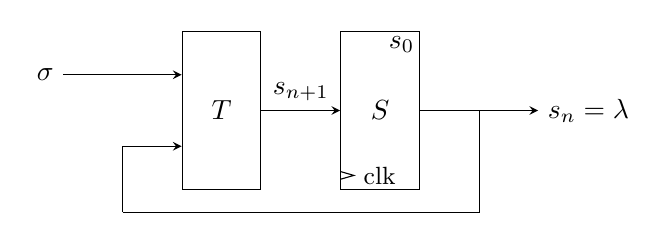
\begin{tikzpicture}

  \node [draw, minimum width=1cm, minimum height=2cm]  (input_logic) {$\bold{T}$};
  \node [draw, minimum width=1cm, minimum height=2cm, right=1cm of input_logic]  (memory) {$\bold{S}$};
  \node [below=0.33cm of input_logic.west]  (input_logic_state_in) {};
  \node [above=0.33cm of input_logic.west]  (input_logic_in_in) {};

  \draw [-stealth] (input_logic.east) -- (memory.west) node[midway,above]{$s_{n+1}$};
  \draw [-stealth] (memory.east) -- ++(1.5,0) node[midway] (state) {} node[behind path, right] {$s_{n} = \lambda$};
  \draw [stealth-] (input_logic_in_in.center) -- ++(-1.5,0) node[midway] (helper1) {} node[behind path, left]{$\sigma$};

  \node [below=1.5cm of helper1]  (helper2) {};
  
  \draw (state.center) |- (helper2.center);
  \draw [-stealth] (helper2.center) |- (input_logic_state_in.center);

  \node [below=0.75cm of memory.west]  (tri_a) {};
  \node [below=0.70cm of memory.west]  (tri_b_) {};
  \node [right=0.05cm of tri_b_.center]  (tri_b) {};
  \node [right=0.00cm of tri_b.center] (clock) {{\small clk}};
  \node [below=0.65cm of memory.west]  (tri_c) {};
  \draw (tri_a.center) -- (tri_b.center)  -- (tri_c.center);

  \node [below=0.05cm of memory.north east]  (s0_) {};
  \node [left=-0.05cm of s0_.center]  (s0) {$s_0$};

  \end{tikzpicture}

\end{center}
  \begin{center}
  \begin{equation}
    s_{n+1} = t(s_n,\sigma)
  \end{equation}
  \begin{equation}
    \lambda = s_n
  \end{equation}
  \end{center}
\end{frame}

\begin{frame}[fragile]{Implementation in Software}
  Procedure
  \begin{itemize}
    \item Define statemachine
    \item choose a statemachine implementation that fits your needs
    \item define the sets matching the process variables ($\bold{S}$, $\bold{\Sigma}$, $\bold{T}$, $\bold{\Lambda}$)
  \end{itemize}
\end{frame}

\begin{frame}[fragile]{}
\begin{center}

      \metroset{block=fill}

      \begin{block}{Experience}
        To properly engineer something you need to understand your components and tools to a certain level.
      \end{block}

      \begin{exampleblock}{Remark}
        Finding that level Depends on the problem.
      \end{exampleblock}

\end{center}
\end{frame}

\section{Titleformats}

\begin{frame}{Metropolis titleformats}
	\themename supports 4 different titleformats:
	\begin{itemize}
		\item Regular
		\item \textsc{Smallcaps}
		\item \textsc{allsmallcaps}
		\item ALLCAPS
	\end{itemize}
	They can either be set at once for every title type or individually.
\end{frame}

\subsection{Tricks}

{
    \metroset{titleformat frame=smallcaps}
\begin{frame}{Small caps}
	This frame uses the \texttt{smallcaps} titleformat.

	\begin{alertblock}{Potential Problems}
		Be aware, that not every font supports small caps. If for example you typeset your presentation with pdfTeX and the Computer Modern Sans Serif font, every text in smallcaps will be typeset with the Computer Modern Serif font instead.
	\end{alertblock}
\end{frame}
}

{
\metroset{titleformat frame=allsmallcaps}
\begin{frame}{All small caps}
	This frame uses the \texttt{allsmallcaps} titleformat.

	\begin{alertblock}{Potential problems}
		As this titleformat also uses smallcaps you face the same problems as with the \texttt{smallcaps} titleformat. Additionally this format can cause some other problems. Please refer to the documentation if you consider using it.

		As a rule of thumb: Just use it for plaintext-only titles.
	\end{alertblock}
\end{frame}
}

{
\metroset{titleformat frame=allcaps}
\begin{frame}{All caps}
	This frame uses the \texttt{allcaps} titleformat.

	\begin{alertblock}{Potential Problems}
		This titleformat is not as problematic as the \texttt{allsmallcaps} format, but basically suffers from the same deficiencies. So please have a look at the documentation if you want to use it.
	\end{alertblock}
\end{frame}
}

\section{Elements}

\begin{frame}[fragile]{Typography}
      \begin{verbatim}The theme provides sensible defaults to
\emph{emphasize} text, \alert{accent} parts
or show \textbf{bold} results.\end{verbatim}

  \begin{center}becomes\end{center}

  The theme provides sensible defaults to \emph{emphasize} text,
  \alert{accent} parts or show \textbf{bold} results.
\end{frame}

\begin{frame}{Font feature test}
  \begin{itemize}
    \item Regular
    \item \textit{Italic}
    \item \textsc{SmallCaps}
    \item \textbf{Bold}
    \item \textbf{\textit{Bold Italic}}
    \item \textbf{\textsc{Bold SmallCaps}}
    \item \texttt{Monospace}
    \item \texttt{\textit{Monospace Italic}}
    \item \texttt{\textbf{Monospace Bold}}
    \item \texttt{\textbf{\textit{Monospace Bold Italic}}}
  \end{itemize}
\end{frame}

\begin{frame}{Lists}
  \begin{columns}[T,onlytextwidth]
    \column{0.33\textwidth}
      Items
      \begin{itemize}
        \item Milk \item Eggs \item Potatos
      \end{itemize}

    \column{0.33\textwidth}
      Enumerations
      \begin{enumerate}
        \item First, \item Second and \item Last.
      \end{enumerate}

    \column{0.33\textwidth}
      Descriptions
      \begin{description}
        \item[PowerPoint] Meeh. \item[Beamer] Yeeeha.
      \end{description}
  \end{columns}
\end{frame}
\begin{frame}{Animation}
  \begin{itemize}[<+- | alert@+>]
    \item \alert<4>{This is\only<4>{ really} important}
    \item Now this
    \item And now this
  \end{itemize}
\end{frame}
\begin{frame}{Figures}
  \begin{figure}
    \newcounter{density}
    \setcounter{density}{20}
    \begin{tikzpicture}
      \def\couleur{alerted text.fg}
      \path[coordinate] (0,0)  coordinate(A)
                  ++( 90:5cm) coordinate(B)
                  ++(0:5cm) coordinate(C)
                  ++(-90:5cm) coordinate(D);
      \draw[fill=\couleur!\thedensity] (A) -- (B) -- (C) --(D) -- cycle;
      \foreach \x in {1,...,40}{%
          \pgfmathsetcounter{density}{\thedensity+20}
          \setcounter{density}{\thedensity}
          \path[coordinate] coordinate(X) at (A){};
          \path[coordinate] (A) -- (B) coordinate[pos=.10](A)
                              -- (C) coordinate[pos=.10](B)
                              -- (D) coordinate[pos=.10](C)
                              -- (X) coordinate[pos=.10](D);
          \draw[fill=\couleur!\thedensity] (A)--(B)--(C)-- (D) -- cycle;
      }
    \end{tikzpicture}
    \caption{Rotated square from
    \href{http://www.texample.net/tikz/examples/rotated-polygons/}{texample.net}.}
  \end{figure}
\end{frame}
\begin{frame}{Tables}
  \begin{table}
    \caption{Largest cities in the world (source: Wikipedia)}
    \begin{tabular}{lr}
      \toprule
      City & Population\\
      \midrule
      Mexico City & 20,116,842\\
      Shanghai & 19,210,000\\
      Peking & 15,796,450\\
      Istanbul & 14,160,467\\
      \bottomrule
    \end{tabular}
  \end{table}
\end{frame}
\begin{frame}{Blocks}
  Three different block environments are pre-defined and may be styled with an
  optional background color.

  \begin{columns}[T,onlytextwidth]
    \column{0.5\textwidth}
      \begin{block}{Default}
        Block content.
      \end{block}

      \begin{alertblock}{Alert}
        Block content.
      \end{alertblock}

      \begin{exampleblock}{Example}
        Block content.
      \end{exampleblock}

    \column{0.5\textwidth}

      \metroset{block=fill}

      \begin{block}{Default}
        Block content.
      \end{block}

      \begin{alertblock}{Alert}
        Block content.
      \end{alertblock}

      \begin{exampleblock}{Example}
        Block content.
      \end{exampleblock}

  \end{columns}
\end{frame}
\begin{frame}{Math}
  \begin{equation*}
    e = \lim_{n\to \infty} \left(1 + \frac{1}{n}\right)^n
  \end{equation*}
\end{frame}
\begin{frame}{Line plots}
  \begin{figure}
    \begin{tikzpicture}
      \begin{axis}[
        mlineplot,
        width=0.9\textwidth,
        height=6cm,
      ]

        \addplot {sin(deg(x))};
        \addplot+[samples=100] {sin(deg(2*x))};

      \end{axis}
    \end{tikzpicture}
  \end{figure}
\end{frame}
\begin{frame}{Bar charts}
  \begin{figure}
    \begin{tikzpicture}
      \begin{axis}[
        mbarplot,
        xlabel={Foo},
        ylabel={Bar},
        width=0.9\textwidth,
        height=6cm,
      ]

      \addplot plot coordinates {(1, 20) (2, 25) (3, 22.4) (4, 12.4)};
      \addplot plot coordinates {(1, 18) (2, 24) (3, 23.5) (4, 13.2)};
      \addplot plot coordinates {(1, 10) (2, 19) (3, 25) (4, 15.2)};

      \legend{lorem, ipsum, dolor}

      \end{axis}
    \end{tikzpicture}
  \end{figure}
\end{frame}
\begin{frame}{Quotes}
  \begin{quote}
    Veni, Vidi, Vici
  \end{quote}
\end{frame}

{%
\setbeamertemplate{frame footer}{My custom footer}
\begin{frame}[fragile]{Frame footer}
    \themename defines a custom beamer template to add a text to the footer. It can be set via
    \begin{verbatim}\setbeamertemplate{frame footer}{My custom footer}\end{verbatim}
\end{frame}
}

\begin{frame}{References}
  Some references to showcase [allowframebreaks] \cite{knuth92,ConcreteMath,Simpson,Er01,greenwade93}
\end{frame}

\section{Conclusion}

\begin{frame}{Summary}

  Get the source of this theme and the demo presentation from

  \begin{center}\url{github.com/matze/mtheme}\end{center}

  The theme \emph{itself} is licensed under a
  \href{http://creativecommons.org/licenses/by-sa/4.0/}{Creative Commons
  Attribution-ShareAlike 4.0 International License}.

  \begin{center}\ccbysa\end{center}

\end{frame}

{\setbeamercolor{palette primary}{fg=black, bg=yellow}
\begin{frame}[standout]
  Questions?
\end{frame}
}

\appendix

\begin{frame}[fragile]{Backup slides}
  Sometimes, it is useful to add slides at the end of your presentation to
  refer to during audience questions.

  The best way to do this is to include the \verb|appendixnumberbeamer|
  package in your preamble and call \verb|\appendix| before your backup slides.

  \themename will automatically turn off slide numbering and progress bars for
  slides in the appendix.
\end{frame}

\begin{frame}[allowframebreaks]{References}

  \bibliography{demo}
  \bibliographystyle{abbrv}

\end{frame}

\end{document}
